\documentclass[border=12pt]{standalone}
\usepackage{tikz}
\usetikzlibrary{shapes.geometric, arrows.meta, positioning, calc, fit, backgrounds}
\usepackage{fontspec}
\setmainfont{DejaVu Sans}

\begin{document}
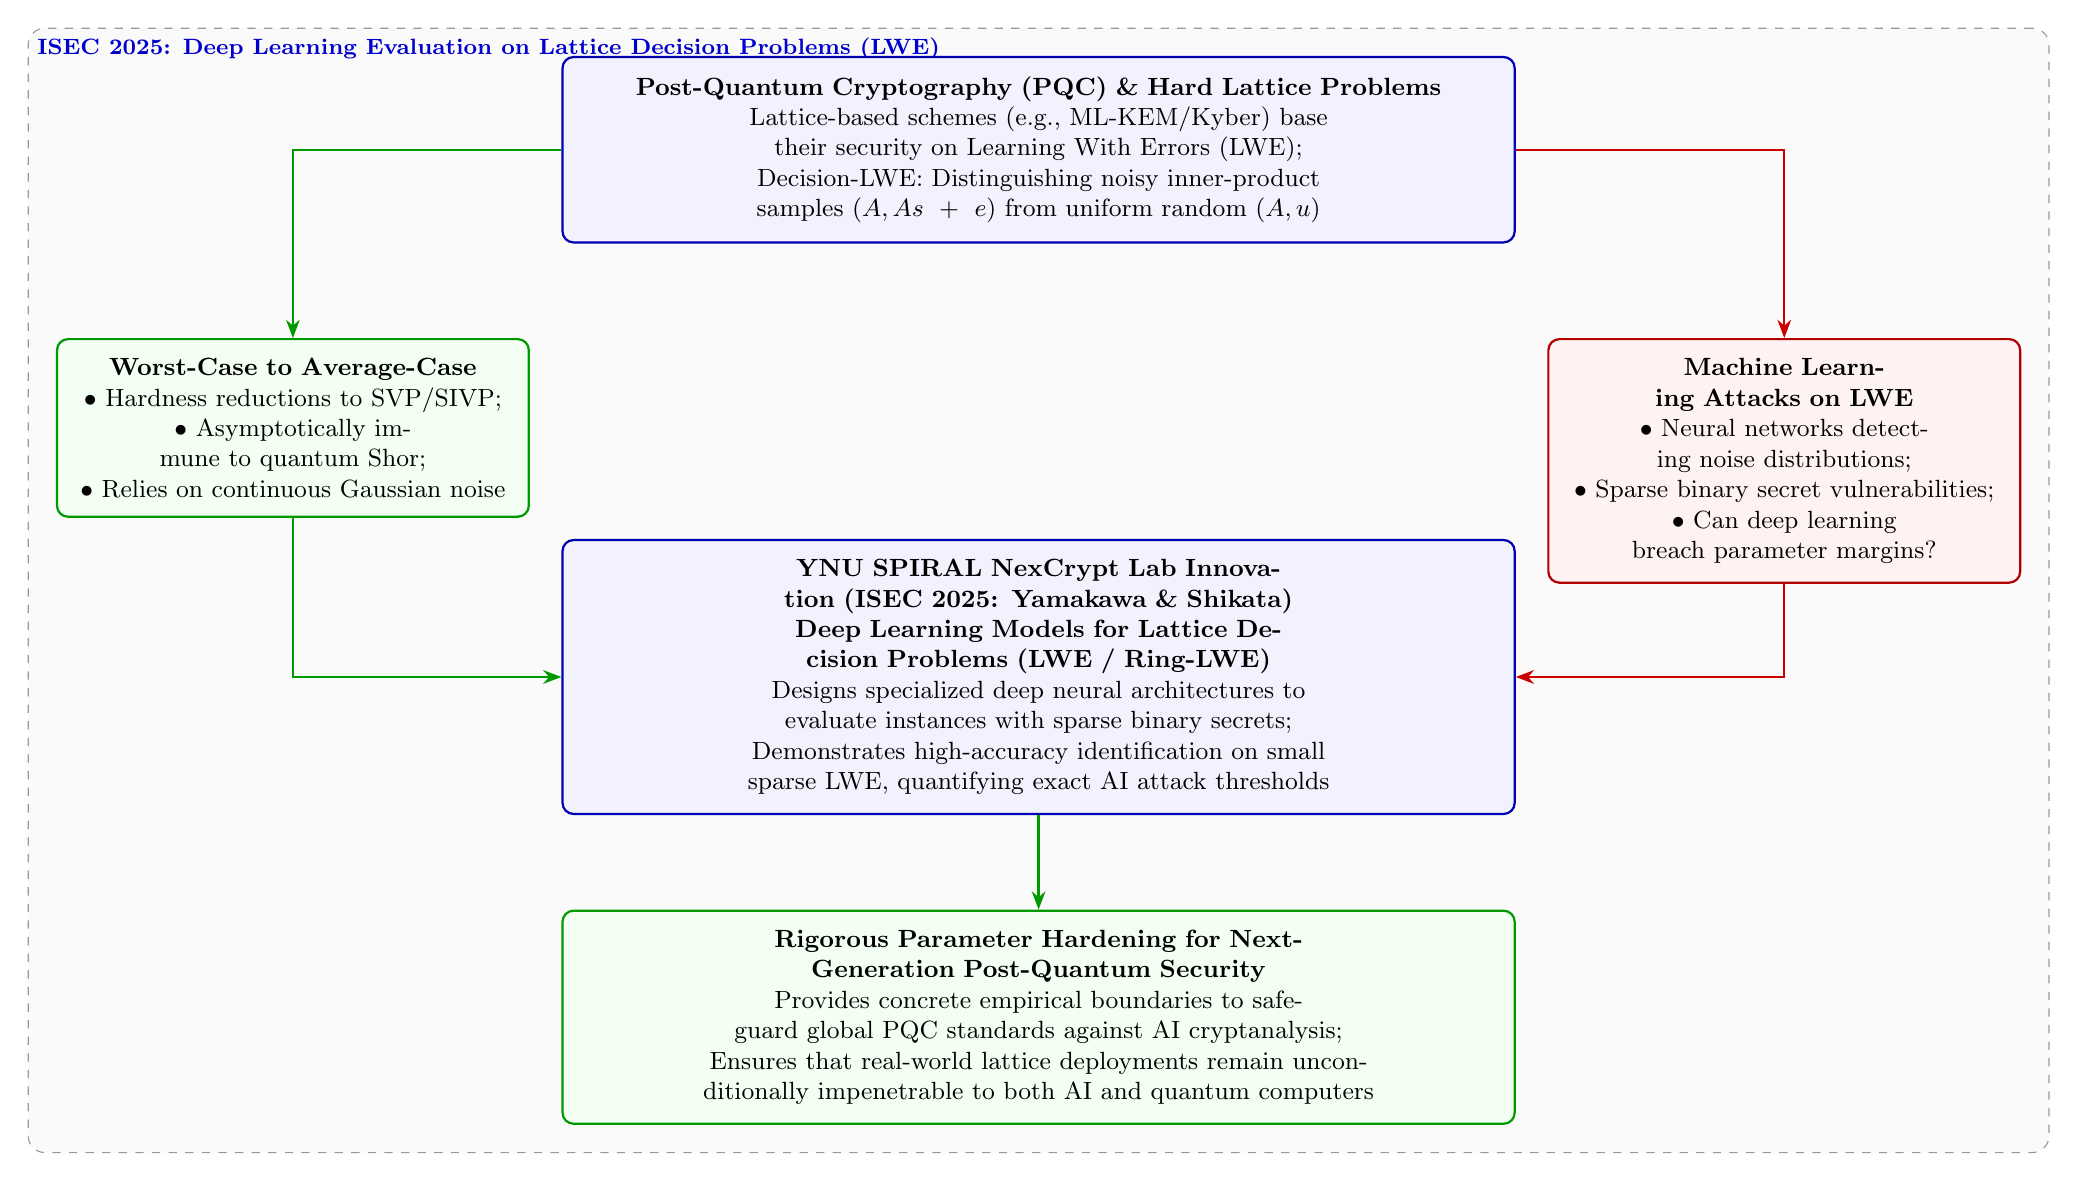
\begin{tikzpicture}[
    font=\small,
    >=Stealth,
    node distance=1.2cm,
    block/.style={rectangle, draw=blue!70!black, fill=blue!5, rounded corners=4pt, thick, align=center, inner sep=7pt},
    alertblock/.style={rectangle, draw=red!70!black, fill=red!5, rounded corners=4pt, thick, align=center, inner sep=7pt},
    greenblock/.style={rectangle, draw=green!60!black, fill=green!5, rounded corners=4pt, thick, align=center, inner sep=7pt},
    amberblock/.style={rectangle, draw=orange!80!black, fill=orange!5, rounded corners=4pt, thick, align=center, inner sep=7pt},
    groupbox/.style={draw=black!40, dashed, rounded corners=6pt, fill=black!2, inner sep=10pt}
]

    % Top: Post-Quantum Cryptography Foundation
    \node[block, text width=11.6cm] (pqc) {\textbf{Post-Quantum Cryptography (PQC) \& Hard Lattice Problems}\\Lattice-based schemes (e.g., ML-KEM/Kyber) base their security on Learning With Errors (LWE);\\Decision-LWE: Distinguishing noisy inner-product samples $(A, As + e)$ from uniform random $(A, u)$};

    % Left: Classical Theoretical Reductions
    \node[greenblock, below left=1.2cm and 0.4cm of pqc, text width=5.5cm] (theory) {\textbf{Worst-Case to Average-Case}\\$\bullet$ Hardness reductions to SVP/SIVP;\\$\bullet$ Asymptotically immune to quantum Shor;\\$\bullet$ Relies on continuous Gaussian noise};

    % Right: Emerging Machine Learning Threat
    \node[alertblock, below right=1.2cm and 0.4cm of pqc, text width=5.5cm] (ai) {\textbf{Machine Learning Attacks on LWE}\\$\bullet$ Neural networks detecting noise distributions;\\$\bullet$ Sparse binary secret vulnerabilities;\\$\bullet$ Can deep learning breach parameter margins?};

    \draw[->, thick, green!60!black] (pqc) -| (theory);
    \draw[->, thick, red!80!black] (pqc) -| (ai);

    % Middle: YNU Discovery (ISEC 2025: Yamakawa & Shikata)
    \node[block, below=1.2cm of $(theory)!0.5!(ai)$, text width=11.6cm] (breakthrough) {\textbf{YNU SPIRAL NexCrypt Lab Innovation (ISEC 2025: Yamakawa \& Shikata)}\\\textbf{Deep Learning Models for Lattice Decision Problems (LWE / Ring-LWE)}\\Designs specialized deep neural architectures to evaluate instances with sparse binary secrets;\\Demonstrates high-accuracy identification on small sparse LWE, quantifying exact AI attack thresholds};

    \draw[->, thick, green!60!black] (theory) |- (breakthrough);
    \draw[->, thick, red!80!black] (ai) |- (breakthrough);

    % Bottom: Impact
    \node[greenblock, below=1.2cm of breakthrough, text width=11.6cm] (impact) {\textbf{Rigorous Parameter Hardening for Next-Generation Post-Quantum Security}\\Provides concrete empirical boundaries to safeguard global PQC standards against AI cryptanalysis;\\Ensures that real-world lattice deployments remain unconditionally impenetrable to both AI and quantum computers};

    \draw[->, thick, green!60!black] (breakthrough) -- (impact);

    \begin{scope}[on background layer]
        \node[groupbox, fit=(pqc) (theory) (ai) (breakthrough) (impact), label={[anchor=north west, font=\footnotesize\bfseries, blue!80!black]north west:ISEC 2025: Deep Learning Evaluation on Lattice Decision Problems (LWE)}] {};
    \end{scope}

\end{tikzpicture}
\end{document}
